\subsection{Semi-automatic modeling for gene regulatory networks} The
common understanding of circadian rhythms is that they are mainly
produced on the transcriptional level by gene regulatory networks,
see~\cite{reppert2002coordination}. When building mathematical models
of such networks, one often stumbles over the large number of poorly
characterized kinetic parameters of the gene regulation and hence is
confronted with a problem of prescribing unknown values to the
numerous numerical parameters of the model. Motivated by an earlier
success of employing delay-differential equations to model circadian
gene regulatory networks (see~\cite{korencic2012interplay}), we
decided to make a further attempt to make such modelling less
supervised and more data-driven.


\begin{figure}
\begin{center}
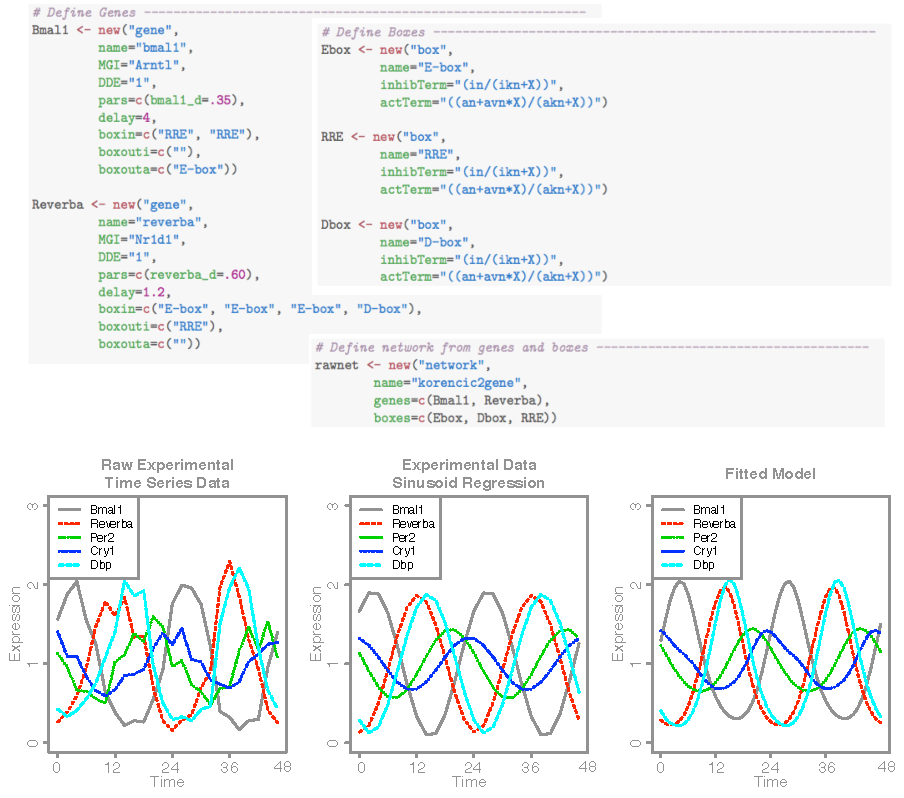
\includegraphics[width=\linewidth]{figures/matt/matt.pdf}
\end{center}
\caption{
  {\bf Upper panel} An example of a human-readable description of a
  gene regulatory network consisting of two genes (Bmal1 and
  Reverb$\alpha$) and three boxes (Ebox, RRE, Dbox).
  {\bf Lower panel} Comparison between oscillations in microarray
  data, the extracted first harmonic and the fit by a model with five
  genes.
\label{fig::matt}
}
\end{figure}

Within his masters dissertation, Matthew
Kondoff~\cite{kondoff2015modeling} looked at a way of automatically
generating computational models from human-readable description of
regulatory gene networks. His efforts resulted in an R package, with
the help of which a convenient way of numerical modeling was
providing, thus hiding the low-level nitty-gritty of translating the
network description into formulas and computer code.


An example description of a simple two-gene, three-box network is
represented in Figure \ref{fig::matt}, upper panel. A highly
human-readable source code in R programming language automatically
produces then an optimized numerical simulation framework with
underlying low-level code for the nonlinear equations in C language
(for performance reasons). As a next step, the unknown parameters of
those nonlinear equations are found to fit the simulated oscillations
(Figure \ref{fig::matt}, lower panel, right plot) to given
experimental data (Figure \ref{fig::matt}, lower panel, left plot).
The data used here came from~\cite{zhang2014circadian}, being a set of
24 microarray assays collected in two hours intervals, totalling 48
hours worth of time series length. Before fitting, the parameters of
the $~$24 hours harmonic were extracted from the data (period,
relative phases and relative amplitudes) and used to define the cost
function in the fitting procedure. For the optimization procedure, the
so-called particle swarm optimzation (see~\cite{zambrano2012hydropso})
was used with optimized initial conditions,
see~\cite{richards2004choosing}.
